% Branching self-play for turn-level DPO — poster flowchart
% Compile: tectonic dpo_selfplay_diagram.tex
\documentclass[tikz,border=8pt]{standalone}
\usetikzlibrary{arrows.meta,fit,backgrounds,shapes.geometric,calc}
\renewcommand{\familydefault}{\sfdefault}

\definecolor{navy}{HTML}{16244F}
\definecolor{blockblue}{HTML}{E3F2FD}
\definecolor{blockblueline}{HTML}{1976D2}
\definecolor{lav}{HTML}{E8EAF6}
\definecolor{lavline}{HTML}{3F51B5}
\definecolor{teal}{HTML}{E0F2F1}
\definecolor{tealline}{HTML}{00897B}
\definecolor{tealdark}{HTML}{00695C}
\definecolor{tealbg}{HTML}{F1FAF9}
\definecolor{amber}{HTML}{FFF8E1}
\definecolor{amberline}{HTML}{F9A825}
\definecolor{orangebg}{HTML}{FFF3E0}
\definecolor{orangeline}{HTML}{EF6C00}
\definecolor{green}{HTML}{E8F5E9}
\definecolor{greenline}{HTML}{2E7D32}
\definecolor{grayfill}{HTML}{FAFAFA}
\definecolor{grayline}{HTML}{9E9E9E}
\definecolor{violet}{HTML}{EDE7F6}
\definecolor{violetline}{HTML}{5E35B1}

\begin{document}
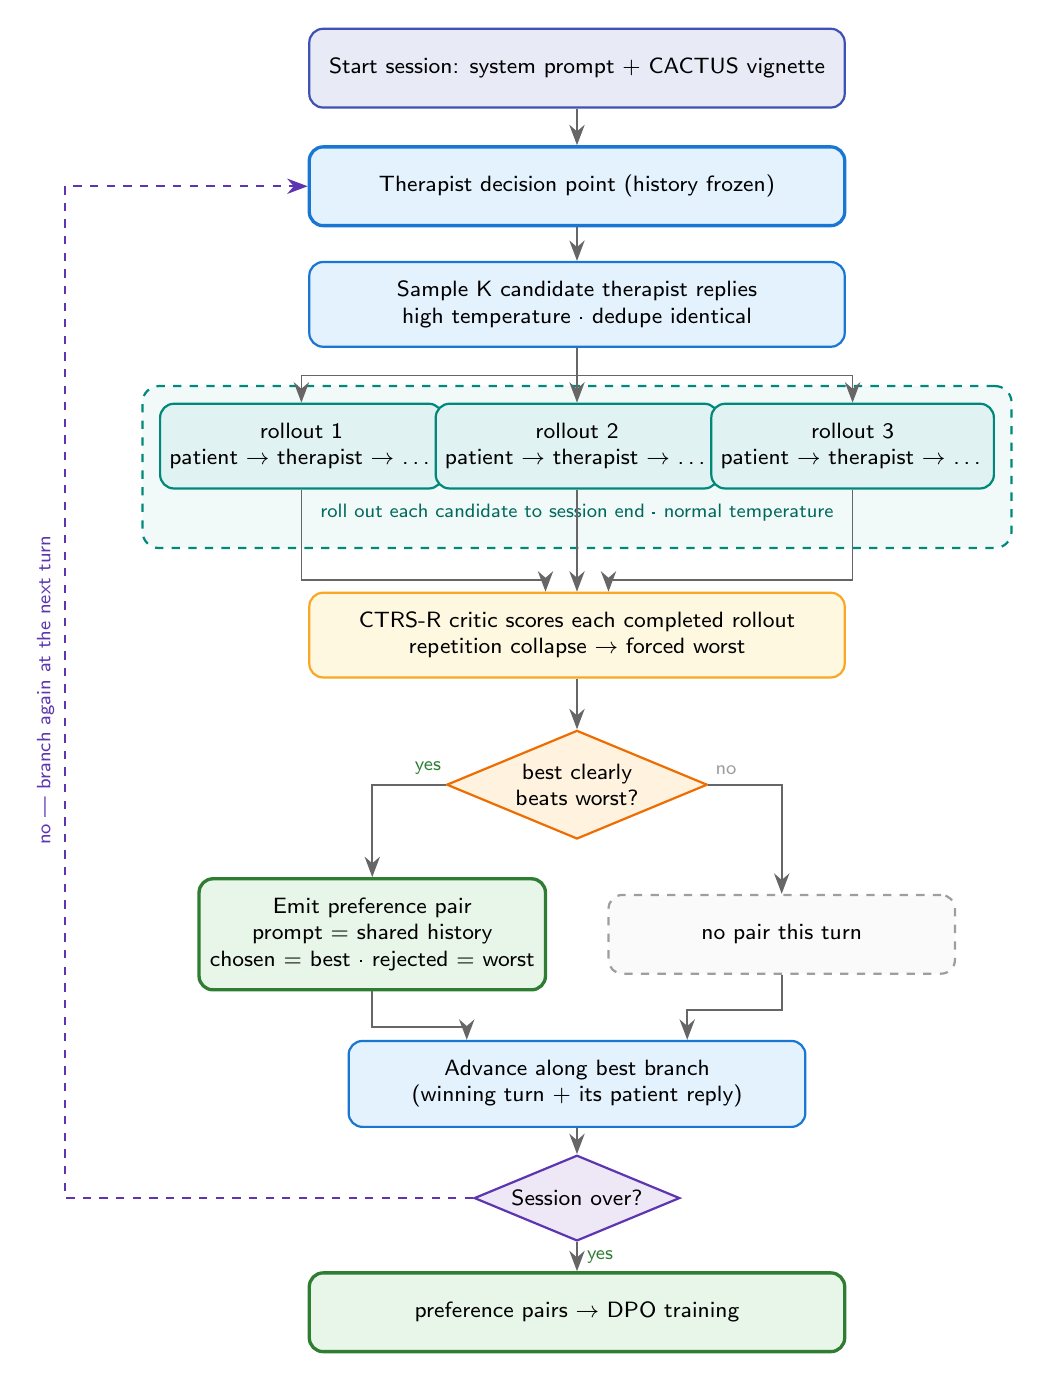
\begin{tikzpicture}[
  block/.style={rounded corners=5pt, draw, thick, align=center,
                font=\footnotesize, inner ysep=7pt, minimum width=68mm,
                minimum height=10mm},
  rblock/.style={block, minimum width=30mm, fill=teal, draw=tealline},
  dec/.style={diamond, aspect=2.4, draw, thick, align=center,
              font=\footnotesize, inner sep=2pt},
  arr/.style={-{Stealth[length=2.6mm]}, draw=black!60, semithick},
  lab/.style={font=\scriptsize},
]

\node[block, fill=lav, draw=lavline] (start) at (0,0)
  {Start session: system prompt + CACTUS vignette};
\node[block, fill=blockblue, draw=blockblueline, very thick] (decision) at (0,-1.5)
  {Therapist decision point (history frozen)};
\node[block, fill=blockblue, draw=blockblueline] (branch) at (0,-3.0)
  {Sample K candidate therapist replies\\ high temperature · dedupe identical};

\node[rblock] (r1) at (-3.5,-4.8) {rollout 1\\ patient $\to$ therapist $\to$ \dots};
\node[rblock] (r2) at (0,-4.8)    {rollout 2\\ patient $\to$ therapist $\to$ \dots};
\node[rblock] (r3) at (3.5,-4.8)  {rollout 3\\ patient $\to$ therapist $\to$ \dots};
\node[font=\scriptsize, text=tealdark] (rcap) at (0,-5.65)
  {roll out each candidate to session end · normal temperature};
\begin{scope}[on background layer]
  \node[fit=(r1)(r3)(rcap), rounded corners=6pt, draw=tealline, dashed,
        thick, fill=tealbg, inner sep=6pt] (cluster) {};
\end{scope}

\node[block, fill=amber, draw=amberline] (judge) at (0,-7.2)
  {CTRS-R critic scores each completed rollout\\ repetition collapse $\to$ forced worst};
\node[dec, fill=orangebg, draw=orangeline] (gate) at (0,-9.1)
  {best clearly\\ beats worst?};
\node[block, minimum width=44mm, fill=green, draw=greenline, very thick] (pair) at (-2.6,-11.0)
  {Emit preference pair\\ prompt = shared history\\ chosen = best · rejected = worst};
\node[block, minimum width=44mm, fill=grayfill, draw=grayline, dashed] (skip) at (2.6,-11.0)
  {no pair this turn};
\node[block, minimum width=58mm, fill=blockblue, draw=blockblueline] (advance) at (0,-12.9)
  {Advance along best branch\\ (winning turn + its patient reply)};
\node[dec, fill=violet, draw=violetline] (done) at (0,-14.35) {Session over?};
\node[block, fill=green, draw=greenline, very thick] (out) at (0,-15.8)
  {preference pairs $\to$ DPO training};

% ── Edges (orthogonal) ──────────────────────────────────────────────────
\draw[arr] (start) -- (decision);
\draw[arr] (decision) -- (branch);
\draw[arr] (branch.south) -- ++(0,-0.35) -| (r1.north);
\draw[arr] (branch.south) -- (r2.north);
\draw[arr] (branch.south) -- ++(0,-0.35) -| (r3.north);
\draw[arr] (r1.south) -- ++(0,-1.15) -| ($(judge.north)+(-0.4,0)$);
\draw[arr] (r2.south) -- (judge.north);
\draw[arr] (r3.south) -- ++(0,-1.15) -| ($(judge.north)+(0.4,0)$);
\draw[arr] (judge) -- (gate);
\draw[arr] (gate.west) -| node[lab, pos=0.12, above, text=greenline] {yes} (pair.north);
\draw[arr] (gate.east) -| node[lab, pos=0.12, above, text=grayline] {no} (skip.north);
\draw[arr] (pair.south) -- ++(0,-0.45) -| ($(advance.north)+(-1.4,0)$);
\draw[arr] (skip.south) -- ++(0,-0.45) -| ($(advance.north)+(1.4,0)$);
\draw[arr] (advance) -- (done);
\draw[arr] (done) -- node[lab, right, text=greenline] {yes} (out);
\draw[arr, dashed, draw=violetline]
  (done.west) -| (-6.5,-1.5) -- (decision.west);
\node[lab, text=violetline, rotate=90] at (-6.75,-7.9) {no — branch again at the next turn};

\end{tikzpicture}
\end{document}
